\documentclass[12pt]{article}
\usepackage[a4paper, top=0.4in, bottom=0.3in, left=0.5in, right=0.5in]{geometry}
\usepackage{graphicx}
\usepackage{subcaption}
\usepackage{listings}
\usepackage{xcolor}
\usepackage{float}
\usepackage{lmodern}
\usepackage[T1]{fontenc}
\usepackage{setspace}
\usepackage{array}
\usepackage{booktabs}
\usepackage{tabularx}
\usepackage{titlesec}
\usepackage{hyperref}

\usepackage{fix-cm}       % allows arbitrary sizes with CM fonts
% \usepackage{xcolor}
\usepackage{tikz}
\usetikzlibrary{decorations.text}

% Sans-serif throughout (like the AI PDF)
\renewcommand{\familydefault}{\sfdefault}

% Hyperref colors
\hypersetup{colorlinks=false}

% Colors matching AI PDF style
\definecolor{rcblue}{RGB}{30, 100, 200}
\definecolor{rcpurple}{RGB}{100, 60, 160}
\definecolor{codegreen}{rgb}{0,0.6,0}
\definecolor{codegray}{rgb}{0.5,0.5,0.5}
\definecolor{codepurple}{rgb}{0.58,0,0.82}
\definecolor{backcolour}{rgb}{0.97,0.97,0.97}

% Code listing style
\lstdefinestyle{mystyle}{
    backgroundcolor=\color{backcolour},
    commentstyle=\color{codegreen},
    keywordstyle=\color{blue}\bfseries,
    numberstyle=\small\color{codegray},
    stringstyle=\color{codepurple},
    basicstyle=\ttfamily\normalsize,
    breaklines=true,
    captionpos=b,
    keepspaces=true,
    numbers=left,
    numbersep=8pt,
    showspaces=false,
    showstringspaces=false,
    tabsize=4,
    xleftmargin=16pt,
    xrightmargin=4pt,
    frame=single,
    framesep=4pt,
    rulecolor=\color{gray!40}
}
\lstset{style=mystyle}

% Section title formatting — bold, large, left-aligned (like AI PDF)
\titleformat{\section}[block]
  {\large\bfseries}
  {\thesection.}
  {0.5em}
  {}
\titlespacing*{\section}{0pt}{18pt}{6pt}

\setlength{\parindent}{0pt}
\setlength{\parskip}{10pt}

\begin{document}

% ============================================================
% TITLE PAGE
% ============================================================
\begin{titlepage}
\centering
% \vspace*{-10pt}

{\fontsize{38pt}{1pt}\selectfont\bfseries Compiler Design Practical}\\[20pt]
% {\fontsize{30pt}{26pt}\selectfont\bfseries\color{purple} UNIVERSITY OF DELHI}\\[10pt]
% \begin{tikzpicture}
%   % Curved text
%   \path[decorate,
%     decoration={
%       text along path,
%       text={|\fontsize{35pt}{26pt}\selectfont\bfseries\color{purple}|UNIVERSITY OF DELHI},
%       text align={center}
%     }
%   ] (0,-2) arc (180:0:5);

%   % Logo at center
%   \node at (5,-.5) {\includegraphics[width=0.30\textwidth]{Ramanujan_logo.png}};
% \end{tikzpicture}

\includegraphics[width=0.75\textwidth]{college_logo.png}\\[26pt]

{\fontsize{28pt}{26pt}\selectfont\bfseries\color{rcblue} Ramanujan College}\\[10pt]

{\fontsize{25pt}{20pt}\selectfont\bfseries\color{rcblue} DSC-19: Compiler Design}\\[10pt]

{\fontsize{25pt}{22pt}\selectfont\bfseries\color{rcblue} Semester-7}\\[10pt]

{\fontsize{20pt}{22pt}\selectfont\bfseries\color{rcblue} (2026-27)}\\[80pt]

\begin{tabular}{p{0.65\textwidth} p{0.48\textwidth}}
{\large\bfseries Submitted By:} & {\large\bfseries Submitted To:} \\[6pt]
{\large\bfseries $\sim$Ratnesh Kumar} & {\large\bfseries $\sim$ Dr.\ Subodh Kumar} \\[3pt]
{\large\bfseries 20231432 (23020570034)} & {\large\bfseries Assistant Professor} \\[3pt]
{\large\bfseries B.Sc.\ (Hons.) CS / VII} & {\large\bfseries Dept.\ of Computer Science} \\
\end{tabular}

\end{titlepage}

% ============================================================
% ACKNOWLEDGEMENT PAGE
% ============================================================
\newpage
\begin{center}
{\fontsize{26pt}{32pt}\selectfont\bfseries Acknowledgement}
\end{center}

\vspace{16pt}
\setstretch{1.5}
{\large
I would like to take this opportunity to acknowledge everyone who has helped me in every stage of this practical work.

I am deeply indebted to my Compiler Design Professor, \textbf{Dr. Subodh Kumar}, Assistant Professor, Department of Computer Science, Ramanujan College, for his valuable guidance, constant encouragement, and suggestions in completing this practical. The completion of this practical was possible under his guidance and support.

I am also thankful to the \textbf{Principal, Ramanujan College}, and the \textbf{Department of Computer Science} for providing the necessary infrastructure and academic environment. I extend my appreciation to all faculty members and laboratory staff who assisted me during the course of this work.

I am also very thankful to my parents and my friends who have boosted me up morally with their continuous support.

At last but not least, I am very thankful to God almighty for showering his blessings upon me.
}
\setstretch{1}

% ============================================================
% INDEX PAGE
% ============================================================
\newpage
\begin{center}
{\fontsize{40pt}{30pt}\selectfont\bfseries\itshape\color{rcblue} Index}
\end{center}

\vspace{10pt}

\renewcommand{\arraystretch}{1.4}
\begin{tabularx}{\textwidth}{|>{\centering\bfseries\large}p{1.5cm}|>{\large}X|}
\hline
\large\bfseries S.no & \centering\large\bfseries Topic \tabularnewline
\hline
1. & Write a Lex program to count the number of lines and characters in the input file. \\
\hline
2. & Write a Lex program to count the number of vowels in a given string. \\
\hline
3. & Write a Lex program that implements the Caesar cipher. \\
\hline
4. & Write a Lex program that finds the longest word in the input. \\
\hline
5. & Write a Lex program that distinguishes keywords, integers, floats, identifiers, operators, and comments. \\
\hline
6. & Write a Lex program to count the number of words, characters, blank spaces and lines in a C file. \\
\hline
7. & Write a Lex specification program that generates a C program which takes a string ``abcd'' and prints a specific pattern. \\
\hline
8. & A program in Lex to recognize a valid arithmetic expression. \\
\hline
9. & Write a YACC program to find the validity of a given expression and recognize a valid variable. \\
\hline
10. & A Program in YACC to evaluate an expression (addition, subtraction, multiplication, division). \\
\hline
11. & Program in YACC to recognize the string `abbb', `ab', `a' of the language $(a^n b^n,\ n\geq 1)$. \\
\hline
12. & Program in YACC to recognize the language $(a^n b,\ n\geq 10)$. \\
\hline
\end{tabularx}

% ============================================================
% PRACTICALS
% ============================================================
\newpage
\pagenumbering{arabic}
\setstretch{1}

%--- Practical 1 ---
\section*{\large\bfseries 1. Write a Lex program to count the number of lines and characters in the input file.}
\addcontentsline{toc}{section}{Practical 1}

\textbf{\large Code:}

\vspace{2pt}
% \textbf{\normalsize practical1.l}
\begin{lstlisting}[language=C]
%{
#include <stdio.h>
int lines = 0;
int chars = 0;
%}

%%
\n      { lines++; chars++; }
.       { chars++; }
%%

int yywrap() {
    return 1;
}

int main() {
    printf("Enter text: ");
    yylex();
    printf("Lines: %d\n", lines);
    printf("Characters: %d\n", chars);
    return 0;
}
\end{lstlisting}

\vspace{8pt}
\textbf{\large Output:}
\begin{figure}[H]
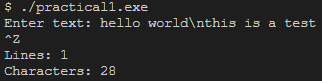
\includegraphics[width=0.60\textwidth]{result/program1_output.png}
\end{figure}

\newpage
%--- Practical 2 ---
\section*{\large\bfseries 2. Write a Lex program to count the number of vowels in a given string.}
\addcontentsline{toc}{section}{Practical 2}

\textbf{\large Code:}

\vspace{4pt}
% \textbf{\normalsize practical2.l}
\begin{lstlisting}[language=C]
%{
#include <stdio.h>
int vowels = 0;
%}

%%
[aeiouAEIOU] { vowels++; }
.            { /* ignore other characters */ }
\n           { /* ignore newlines */ }
%%

int yywrap() {
    return 1;
}

int main() {
    printf("Enter a string: ");
    yylex();
    printf("Number of vowels: %d\n", vowels);
    return 0;
}
\end{lstlisting}

\vspace{8pt}
\textbf{\large Output:}
\begin{figure}[H]
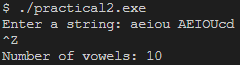
\includegraphics[width=0.60\textwidth]{result/program2_output.png}
\end{figure}

\newpage
%--- Practical 3 ---
\section*{\large\bfseries 3. Write a Lex program that implements the Caesar cipher.}
\addcontentsline{toc}{section}{Practical 3}

\textbf{\large Code:}

\vspace{4pt}
% \textbf{\normalsize practical3.l}
\begin{lstlisting}[language=C]
%{
#include <stdio.h>
%}

%%
[a-w]   { printf("%c", yytext[0] + 3); }
[x-z]   { printf("%c", yytext[0] - 23); }
[A-W]   { printf("%c", yytext[0] + 3); }
[X-Z]   { printf("%c", yytext[0] - 23); }
.|\n    { printf("%c", yytext[0]); }
%%

int yywrap() {
    return 1;
}

int main() {
    printf("Enter text to encrypt using Caesar cipher (shift by 3): ");
    yylex();
    return 0;
}
\end{lstlisting}

\vspace{8pt}
\textbf{\large Output:}
\begin{figure}[H]
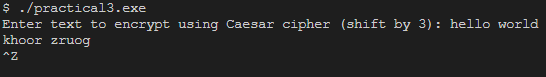
\includegraphics[width=0.65\textwidth]{result/program3_output.png}
\end{figure}

\newpage
%--- Practical 4 ---
\section*{\large\bfseries 4. Write a Lex program that finds the longest word in the input.}
\addcontentsline{toc}{section}{Practical 4}

\textbf{\large Code:}

\vspace{2pt}
% \textbf{\normalsize practical4.l}
\begin{lstlisting}[language=C]
%{
#include <stdio.h>
#include <string.h>

int max_len = 0;
char longest_word[100];
%}

%%
[a-zA-Z]+ { 
    if (yyleng > max_len) {
        max_len = yyleng;
        strcpy(longest_word, yytext);
    }
}
.|\n { /* ignore other characters */ }
%%

int yywrap() {
    return 1;
}

int main() {
    printf("Enter text: ");
    yylex();

    if (max_len > 0) {
        printf("Longest word is '%s' with length %d\n", longest_word, max_len);
    } else {
        printf("No words found.\n");
    }
    return 0;
}
\end{lstlisting}

\vspace{8pt}
\textbf{\large Output:}
\begin{figure}[H]
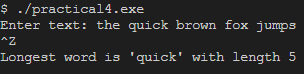
\includegraphics[width=0.65\textwidth]{result/program4_output.png}
\end{figure}

\newpage
%--- Practical 5 ---
\section*{\large\bfseries 5. Write a Lex program that distinguishes keywords, integers, floats, identifiers, operators, and comments.}
\addcontentsline{toc}{section}{Practical 5}

\textbf{\large Code:}

\vspace{2pt}
% \textbf{\normalsize practical5.l}
\begin{lstlisting}[language=C]
%{
#include <stdio.h>
%}

%%
"int"|"float"|"char"|"if"|"else"|"while"|"for"|"return" { printf("Keyword: %s\n", yytext); }
[0-9]+\.[0-9]+          { printf("Float: %s\n", yytext); }
[0-9]+                  { printf("Integer: %s\n", yytext); }
[a-zA-Z_][a-zA-Z0-9_]*  { printf("Identifier: %s\n", yytext); }
"+"|"-"|"*"|"/"|"="     { printf("Operator: %s\n", yytext); }
"//".*                  { printf("Single-line comment: %s\n", yytext); }
"/*"([^*]|\*+[^*/])*\*+"/" { printf("Multi-line comment\n"); }
[ \t\n]                 { /* Ignore whitespace */ }
.                       { printf("Unknown character: %s\n", yytext); }
%%

int yywrap() {
    return 1;
}

int main() {
    printf("Enter code: ");
    yylex();
    return 0;
}
\end{lstlisting}

\vspace{8pt}
\textbf{\large Output:}
\begin{figure}[H]
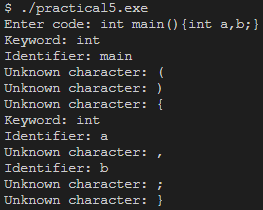
\includegraphics[width=0.60\textwidth]{result/program5_output.png}
\end{figure}

\newpage
%--- Practical 6 ---
\section*{\large\bfseries 6. Write a Lex program to count the number of words, characters, blank spaces and lines in a C file.}
\addcontentsline{toc}{section}{Practical 6}

\textbf{\large Code:}

\vspace{2pt}
% \textbf{\normalsize practical6.l}
\begin{lstlisting}[language=C]
%{
#include <stdio.h>
int words = 0;
int chars = 0;
int blanks = 0;
int lines = 0;
%}

%%
[a-zA-Z_][a-zA-Z0-9_]* { words++; chars += yyleng; }
[ \t]                  { blanks++; chars++; }
\n                     { lines++; chars++; }
.                      { chars++; }
%%

int yywrap() {
    return 1;
}

int main() {
    printf("Enter C code: ");
    yylex();

    printf("Lines: %d\n", lines);
    printf("Words: %d\n", words);
    printf("Blank spaces: %d\n", blanks);
    printf("Characters: %d\n", chars);

    return 0;
}
\end{lstlisting}

\vspace{8pt}
\textbf{\large Output:}
\begin{figure}[H]
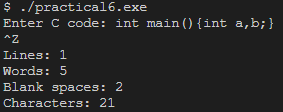
\includegraphics[width=0.50\textwidth]{result/program6_output.png}
\end{figure}

\newpage
%--- Practical 7 ---
\section*{\large\bfseries 7. Write a Lex specification program that generates a C program which takes a string ``abcd'' and prints a specific pattern.}
\addcontentsline{toc}{section}{Practical 7}

\textbf{\large Code:}

\vspace{4pt}
% \textbf{\normalsize practical7.l}
\begin{lstlisting}[language=C]
%{
#include <stdio.h>
#include <string.h>
%}

%%
"abcd" {
    int len = yyleng;
    for (int i = 0; i < len; i++) {
        for (int j = 0; j < len - i; j++) {
            printf("%c", yytext[j]);
        }
        printf("\n");
    }
}
.|\n { /* ignore other inputs */ }
%%

int yywrap() {
    return 1;
}

int main() {
    printf("Enter string 'abcd': ");
    yylex();
    return 0;
}
\end{lstlisting}

\vspace{8pt}
\textbf{\large Output:}
\begin{figure}[H]
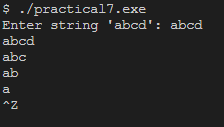
\includegraphics[width=0.45\textwidth]{result/program7_output.png}
\end{figure}

\newpage
%--- Practical 8 ---
\section*{\large\bfseries 8. A program in Lex to recognize a valid arithmetic expression.}
\addcontentsline{toc}{section}{Practical 8}

\textbf{\large Code:}

\vspace{4pt}
% \textbf{\normalsize practical8.l}
\begin{lstlisting}[language=C]
%{
#include <stdio.h>
int op = 0;
int id = 0;
int valid = 1;
%}

%%
[a-zA-Z0-9]+    { id++; printf("Operand\n"); }
[+\-*/]         { op++; printf("Operator\n"); }
[ \t\n]         { /* ignore */ }
.               { valid = 0; }
%%

int yywrap() {
    return 1;
}

int main() {
    printf("Enter an arithmetic expression: ");
    yylex();
    
    if (valid && id == op + 1 && id >= 1) {
        printf("Valid Arithmetic Expression\n");
    } else {
        printf("Invalid Arithmetic Expression\n");
    }
    return 0;
}
\end{lstlisting}

\vspace{8pt}
\textbf{\large Output:}
\begin{figure}[H]
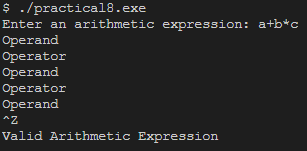
\includegraphics[width=0.55\textwidth]{result/program8_output.png}
\end{figure}

\newpage
%--- Practical 9 ---
\section*{\large\bfseries 9. Write a YACC program to find the validity of a given expression and recognize a valid variable.}
\addcontentsline{toc}{section}{Practical 9}

\textbf{\large Code:}

\vspace{4pt}
\textbf{\normalsize Lex Source File}
\begin{lstlisting}[language=C]
%{
#include "y.tab.h"
%}

%%
[a-z][0-9]      { return VAR; }
[0-9]+          { return NUM; }
[+\-*/()]       { return yytext[0]; }
\n              { return '\n'; }
[ \t]           { /* ignore whitespace */ }
.               { return yytext[0]; }
%%

int yywrap() {
    return 1;
}
\end{lstlisting}

\vspace{8pt}
\textbf{\normalsize Yacc Source File}
\begin{lstlisting}[language=C]
%{
#include <stdio.h>
#include <stdlib.h>
int yylex();
void yyerror(const char *s);
%}

%token VAR NUM

%left '+' '-'
%left '*' '/'

%%
lines:  /* empty */
        | lines expr '\n' { printf("Valid Expression\n"); }
        | lines error '\n' { yyerrok; }
        ;

expr:   VAR
        | NUM
        | expr '+' expr
        | expr '-' expr
        | expr '*' expr
        | expr '/' expr
        | '(' expr ')'
        ;
%%

void yyerror(const char *s) {
    printf("Invalid Expression\n");
}

int main() {
    printf("Enter expression (e.g., a1 + 5): ");
    yyparse();
    return 0;
}
\end{lstlisting}

\vspace{8pt}
\textbf{\large Output:}
\begin{figure}[H]
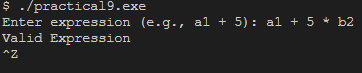
\includegraphics[width=0.65\textwidth]{result/program9_output.png}
\end{figure}

\newpage
%--- Practical 10 ---
\section*{\large\bfseries 10. A Program in YACC to evaluate an expression (addition, subtraction, multiplication, division).}
\addcontentsline{toc}{section}{Practical 10}

\textbf{\large Code:}

\vspace{4pt}
\textbf{\normalsize Lex Source File}
\begin{lstlisting}[language=C]
%{
#include "y.tab.h"
#include <stdlib.h>
%}

%%
[0-9]+          { yylval = atoi(yytext); return NUM; }
[+\-*/()]       { return yytext[0]; }
\n              { return '\n'; }
[ \t]           { /* ignore whitespace */ }
.               { return yytext[0]; }
%%

int yywrap() {
    return 1;
}
\end{lstlisting}

\vspace{8pt}
\textbf{\normalsize Yacc Source File}
\begin{lstlisting}[language=C]
%{
#include <stdio.h>
#include <stdlib.h>
int yylex();
void yyerror(const char *s);
%}

%token NUM

%left '+' '-'
%left '*' '/'

%%
lines:  /* empty */
        | lines expr '\n' { printf("Result = %d\n", $2); }
        | lines error '\n' { yyerrok; }
        ;

expr:   NUM             { $$ = $1; }
        | expr '+' expr { $$ = $1 + $3; }
        | expr '-' expr { $$ = $1 - $3; }
        | expr '*' expr { $$ = $1 * $3; }
        | expr '/' expr { 
            if ($3 == 0) {
                yyerror("Division by zero");
                $$ = 0;
            } else {
                $$ = $1 / $3;
            }
        }
        | '(' expr ')'  { $$ = $2; }
        ;
%%

void yyerror(const char *s) {
    printf("Error: %s\n", s);
}

int main() {
    printf("Enter an arithmetic expression to evaluate: ");
    yyparse();
    return 0;
}
\end{lstlisting}

\vspace{8pt}
\textbf{\large Output:}
\begin{figure}[H]
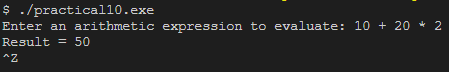
\includegraphics[width=0.65\textwidth]{result/program10_output.png}
\end{figure}

\newpage
%--- Practical 11 ---
\section*{\large\bfseries 11. Program in YACC to recognize the string `abbb', `ab', `a' of the language $(a^n b^n,\ n\geq 1)$.}
\addcontentsline{toc}{section}{Practical 11}

\textbf{\large Code:}

\vspace{4pt}
\textbf{\normalsize Lex Source File}
\begin{lstlisting}[language=C]
%{
#include "y.tab.h"
%}

%%
a       { return A; }
b       { return B; }
\n      { return '\n'; }
.       { return yytext[0]; }
%%

int yywrap() {
    return 1;
}
\end{lstlisting}

\vspace{8pt}
\textbf{\normalsize Yacc Source File}
\begin{lstlisting}[language=C]
%{
#include <stdio.h>
#include <stdlib.h>
int yylex();
void yyerror(const char *s);
%}

%token A B

%%
lines:  /* empty */
        | lines S '\n' { printf("Valid string for a^n b^n\n"); }
        | lines error '\n' { yyerrok; }
        ;

S:      A B
        | A S B
        ;
%%

void yyerror(const char *s) {
    printf("Invalid string\n");
}

int main() {
    printf("Enter string (e.g., ab, aabb, aaabbb): ");
    yyparse();
    return 0;
}
\end{lstlisting}

\vspace{8pt}
\textbf{\large Output:}
\begin{figure}[H]
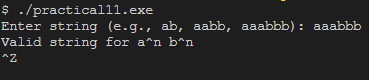
\includegraphics[width=0.65\textwidth]{result/program11_output.png}
\end{figure}

\newpage
%--- Practical 12 ---
\section*{\large\bfseries 12. Program in YACC to recognize the language $(a^n b,\ n\geq 10)$.}
\addcontentsline{toc}{section}{Practical 12}

\textbf{\large Code:}

\vspace{4pt}
\textbf{\normalsize Lex Source File}
\begin{lstlisting}[language=C]
%{
#include "y.tab.h"
%}

%%
a       { return A; }
b       { return B; }
\n      { return '\n'; }
.       { return yytext[0]; }
%%

int yywrap() {
    return 1;
}
\end{lstlisting}

\vspace{8pt}
\textbf{\normalsize Yacc Source File}
\begin{lstlisting}[language=C]
%{
#include <stdio.h>
#include <stdlib.h>
int yylex();
void yyerror(const char *s);
%}

%token A B

%%
lines:  /* empty */
        | lines S '\n' { printf("Valid string for a^n b, n>=10\n"); }
        | lines error '\n' { yyerrok; }
        ;

S:      A A A A A A A A A A A_list B
        ;

A_list: /* empty */
        | A A_list
        ;
%%

void yyerror(const char *s) {
    printf("Invalid string\n");
}

int main() {
    printf("Enter string (e.g., aaaaaaaaaab, aaaaaaaaaaab): ");
    yyparse();
    return 0;
}
\end{lstlisting}

\vspace{8pt}
\textbf{\large Output:}
\begin{figure}[H]
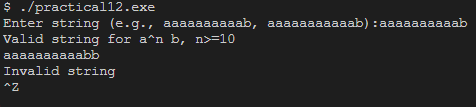
\includegraphics[width=0.65\textwidth]{result/program12_output.png}
\end{figure}

\end{document}
